\documentclass[conference]{IEEEtran}
\IEEEoverridecommandlockouts
% The preceding line is only needed to identify funding in the first footnote. If that is unneeded, please comment it out.
\usepackage{cite}
\usepackage{amsmath,amssymb,amsfonts}
\usepackage[english,russian]{babel}
\usepackage{algorithmic}
\usepackage{graphicx}
\usepackage{hyperref}
\usepackage{textcomp}
\usepackage{xcolor}
\def\BibTeX{{\rm B\kern-.05em{\sc i\kern-.025em b}\kern-.08em
    T\kern-.1667em\lower.7ex\hbox{E}\kern-.125emX}}
\begin{document}

\title{Анализ поездок на ж/д транспорте по России}

\author{\IEEEauthorblockN{Соломатин Макар}
\IEEEauthorblockA{\textit{СПб ПУ} \\
Санкт-Петербург, Россия \\
topdoggyp@gmail.com}
\and
\IEEEauthorblockN{Дамаскинский Константин}
\IEEEauthorblockA{\textit{СПб ПУ} \\
Санкт-Петербург, Россия \\
damaskinsk@mail.ru}}

\maketitle

\begin{abstract}
Данный отчёт посвящён проекту о сборе и анализе данных о железнодорожных поездках по России. В ходе реализации проекта был произведён сбор и анализ данных о продажах билетов на поезда дальнего следования. Предложена система горизонтального масштабирования сбора и анализа данных.
\end{abstract}

Ключевые слова -- большие данные, поезд дальнего следования, динамическое ценообразование, РЖД


\section{Введение}
В настоящее время в России основным пассажирским перевозчиком в железнодорожном сообщении на дальние расстояния (более 200 км) является ПАО ``РЖД''. Помимо государственной ``РЖД'' существует всего два частных перевозчика: ООО ``Тверской экспресс'', владеющий курсирующим между двумя столицами ``Мегаполисом'', и АО ТК ``Гранд Сервис Экспресс'', которое управляет поездами ``Таврия'', курсирующими из разных городов России в Крым, и поездом ``Гранд Экспресс'', совершающим рейсы из Петербурга в Москву. При этом информация о \textbf{всех} поездах, следующих по территории РФ, как принадлежащих РЖД, так и нет, размещена на сайте \href{https://rzd.ru}{https://rzd.ru}.

АО ``РЖД'' устанавливает цены на билеты с использованием программы \textbf{динамического ценообразования}. Это означает, что цена на билет постоянно меняется, начиная с дня открытия продаж (за 90 дней до отправления поезда) и заканчивая днём отправления поезда. Цена билета зависит от множества факторов: времени до отправления поезда, количества свободных мест, скорости покупки билетов, дня недели, близости праздников, времени года и многих других факторов.

Согласно статистике РЖД (\href{https://company.rzd.ru/ru/9377}{https://company.rzd.ru/ru/9377}), за период с января по ноябрь 2021 года РЖД перевезено 85,3 млн человек в дальнем следовании, что составляет в среднем 7.8 млн человек в месяц или 258 тысяч человек в день.

Совокупность указанных фактов позволяет сделать вывод о том, что анализ ценовой политики ``РЖД'' является очень востребованным и будет полезен для огромного количества путешественников.

\section{Цели и задачи проекта}

\subsection{Цели проекта}
Данная работа, как учебный проект, в первую очередь преследует целью получение опыта в анализе больших объёмов данных. Производственные цели проекта -- это, во-первых, исследование политики динамического ценообразования РЖД, и, во-вторых, исследование потребительских трендов в сфере ж/д перевозок.

\subsection{Задачи проекта}

Для достижения поставленных целей необходимо решить задачи:
\begin{itemize}
	\item Получение доступа к источнику данных, отбор наиболее интересной для исследования информации
	\item Разработка системы горизонтального масштабирования сбора данных
	\item Анализ сбора данных
	\item Создание дистрибутива
\end{itemize} 

\subsection{Аналитические задачи}

В рамках данного проекта необходимо проанализировать программу динамического ценообразования РЖД. В текущей версии проекта исследуется зависимость стоимости билетов на поезд от количества дней до отправления поезда и зависимость количества свободных мест от количества дней до отправления поезда. Анализ первой и второй зависимости в совокупности позволяет судить о том, как меняется стоимость билета на поезд в зависимости от потребительского спроса. Анализ второй зависимости позволяет понять, в какие дни пассажиры наиболее активно скупают билеты на поезд, а также как РЖД решает проблему дефицита мест: есть ли смысл ждать добавления дополнительного вагона, или же надо сразу покупать билет на более дорогой поезд либо в более дорогой класс вагона.

Наиболее интересными представляются зависимости стоимости от количества дней до отправления, в которых отношение максимальной и минимальной цены за весь период продаж наибольшее, поскольку именно в таких ситуациях наше исследование является наиболее востребованным. На данных графиках мы будем обращать внимание на дни, в которые стоимость билетов максимальна и минимальна, и на характер изменения цены (в какие периоды растёт, в какие падает). Поскольку работа делается в канун нового года (периода крайне высокой пассажирской активности), обозначенные исследования будут проведены для дат отправления в непосредственной близости праздников (27-30 декабря), а также задолго до праздников и сразу после них. Такая совокупность исследований также позволит выбрать наиболее удачные дни непосредственно для совершения поездки.

\section{Обзор и исследование аналогичных решений}

Для исследования программы динамического ценообразования в первую очередь следует обратиться на сайт РЖД. Корпорация описывает только общие черты программы: ``Система в реальном времени анализирует сотни различных факторов и в зависимости от полученных данных периодически производит перерасчет стоимости проезда по всему маршруту следования. В результате цена билета может измениться в течение часа и даже нескольких минут''.
% TODO ссылка
Кроме того, РЖД демонстрирует ценообразование для пяти популярных маршрутов, связывающих Москву с Санкт-Петербургом, Адлером, Белгородом и Самарой. На приведённых диаграммах показано, за сколько дней до отправления лучше всего покупать билеты, как меняется средняя стоимость в зависимости от дня недели, а также в какое время года поездку можно совершить наиболее выгодно. % TODO ссылка
Из приведённых графиков видно, что наиболее выгодным сезоном для поездки является зима, а наиболее дорогим -- лето. Также можно наблюдать, что цены значительно выше в выходные дни, а билеты лучше всего покупать заранее. При этом для южного направления понятие ``заранее'' является гораздо более жёстким, чем для остальных: покупая билет за целых 60 дней до отправления поезда, пассажир переплачивает 22\% по сравнению со стоимостью за 90 дней до отправления, в то время как для остальных маршрутов существенно динамичным периодом ценообразования является последний месяц продажи билетов.

Альтернативных хоть сколько-нибудь строгих исследований найдено не было. Так, журнал ``Тинькоффа'' % TODO ссылка
даёт лишь общие рекомендации по покупке билетов. Авторы статьи советуют следить за календарём тарифов, который отображает процент повышения цены в каждом месяце, и выбирать наименее популярное время и дату отправления для дополнительной экономии денег. Другие найденные статьи советуют производить аналогичные манипуляции при выборе билета.

\section{Описание модели данных и характеристикаи датасета}
\subsection{Характеристики данных}

Для сбора исследуемых данных авторы используют web-запросы к сайту РЖД. Собираются данные о поездах, следующих между всеми парами из топ 100 городов по численности населения, то есть запросы о 10000 парах городах. Важно заметить, что далеко не все упомянутые пары городов связаны железной дорогой, поэтому в итоге мы получаем значительно меньше, чем 10000 пар городов. Данные собираются каждый день, поскольку необходимо отслеживать динамику изменения цен на билеты. РЖД присылает данные о поездах в формате JSON. На данный момент собрано %TODO сколько???
гигабайт данных.

\subsection{Особенности процесса сбора данных}

\subsubsection{API РЖД}
Первая трудность, с которой столкнулись авторы, это полное отсутствие документации по API РЖД. Нами был найден проект энтузиаста, который создал API на PHP и описал последовательность запросов, которую необходимо совершить для получения требуемых данных. % TODO ссылка

Было установлено, что для получения информации о поездах между указанными парами городов необходимо совершить двухэтапный запрос. На первом этапе отправляются данные о дате отправления и кодах АСУ Экспресс-3 станций отправления и прибытия. В ответ на данный запрос РЖД присылает уникальный идентификатор запроса RID, по которому можно один раз в течение некоторого периода времени совершить второй запрос и получить запрошенные данные. В результате экспериментов было выяснено, что для корректной работы данной схемы между запросами требуется выдержать ``магический интервал'' в 3 секунды.

В ходе сбора данных авторы выяснили, что РЖД отслеижвает число одновременных запросов с одного IP-адреса. В результате ряда экспериментов был сделанвывод о том, что после 15 одновременных запросов с одного IP адреса сайт РЖД отказывает в выполнении последующих запросов приблизительно на 10 минут. Максимально допустимое количество одновременных запросов меняется в зависимости от нагрузки на сайт, и может составлять от 10 до 30 запросов.

Получив данные сведения, авторы приняли решение использовать proxy-сервера для увеличения количества возможных одновременных запросов. В текущей версии проекта нами используется 25 прокси-серверов, что позволяет исполнять в среднем 375 одновременных запросов.

\subsubsection{Ограничения на доступ к данным}
Список дат, на которые можно получить информацию о продажах билетов, ограничен. Так, нельзя получить сведения о поездах, которые отправились до даты сборы, либо позднее, чем 90 дней после неё, то есть информацию о поезде можно получить непосредственно в период продажи билетов на него. Из-за этого размер датасета, который могут собрать авторы, значительно ограничен, и его необходимо пополнять каждый день.


\subsubsection{Неконсистентность данных}
Часто оказывается, что название станции не совпадает с названием города. Поскольку исследование касается путешествий именно между городами, а не между станциями, необходимо сопоставлять название города и всех станций на его территории, с которых отправляются поезда. В решении этой проблемы помогает специальный сервис РЖД %TODO ссылка
. 

Неконсистентность данных также встречается, когда РЖД изменяет конечные станции следования поездов. Например, в 2021 году в Москве открылся новый вокзал ``Восточный'', и 12 декабря поезд 071В поменял начальную станцию с Москва-Курская на Москва-Восточная. Данный поезд идёт через Тулу и Курск, и в результате изменения расписания получилась такая ситуация, когда в один и тот же день между этими городами следует два поезда с одним номером, хотя предполагается, что один поезд идёт не чаще, чем раз в день.

\subsection{Этапы сбора данных}

Сбор данных начинается с получения списка интересующих городов. ДЛя этого была взята статья на Википедии %TODO ссылка
, содержащая таблицу российских городов и их населения. Далее необходимо получить коды АСУ Экспресс-3 для станций в интересующих городах.

Затем ежедневно для каждой пары городов и для всех дат в 90-дневный период, начиная с текущего дня, необходимо сделать запросы списка поездов с билетами. Полученные данные сохраняются в JSON-формате, затем выделяются необходимые данные и отправляются в базу данных MongoDB.

\section{Предлагаемое программное решение}

Программные модули проекта реализованы на языке Python версии 3.10. Проект состоит из нескольких пакетов.

\begin{enumerate}
	\item Пакет collect собирает данные по всем интересующим поездам на ближайшие 90 дней
	
	\item Пакет export отправляет собранные данные в базу данных MongoDB
	
	\item Пакет database совершает запросы к базе данных и локальному хранилищу. В пакете реализован общий интерфейс, перегрузив который можно при необходимости добавлять другие хранилища данных о билетах.
	
	\item Пакет process производит аналитику данных в двух режимах:
	
	\begin{itemize}
		\item Локально с использованием многопоточности (используется количество потоков, равное количеству ядер процессора)
		
		\item С подключением к кластеру Apache Spark (можно использовать любое количество worker-ов)
	\end{itemize}
\end{enumerate}

\section{Описание реализации и технологий}

\subsection{Стек технологий}
Сбор данных производится с использованием Python 3.10 и брокера сообщений Rabbit MQ, в который посылаются задачи по сбору данных. Rabbit MQ необходим, когда сбор данных осуществляется не только с использованием нескольких proxy-серверов, но и на разных физических машинах (когда пропускной способности сетевой карты одного компьютера перестаёт хватать). Обработка данных также производится на Python 3.10 с использованием многопоточности или фреймворка Apache Spark. В качестве системы контроля версий используется git, удалённый репозиторий размещён на github % TODO ссылка
Система управления базами данных -- MongoDB.

\subsection{Горизонтальное масштабирование}

Данный проект поддерживает горизонтальное масштабирование как при сборе, так и при обработке данных. Сбор данных можно осуществлять на нескольких физических машинах с использованием брокера сообщений RabbitMQ. При обработке данных горизонтальное масштабирование осуществляется посредством увеличения числа Spark worker-ов.

\subsection{Состав дистрибутива}

Дистрибутив представляет из себя набора Python пакетов. Для каждого пакета существует свой Dockerfile. Также в дистрибутив входит файл со списком кодов и названий станций, файл с настройками используемых proxy-сервеов (для каждого пользователя свой).

Для развёртывания всей инфраструктуры в локальных контейнерах используется Docker compose. Для развёртывания всего проекта используется Makefile.

Дистрибутив доступен по ссылке. %TODO ссылка

\subsection{Инфраструктура разработки}

Для организации процесса распределённого сбора и обработки данных используется Яндекс.Облако. Зайдействованы 3 виртуальные машины, содержащие 2 ядра Intel Cascad Lake с гарантированной долей CPU 10\%, 4 Гб оперативной памяти и жёсткий диск на 20 Гб. Данные сохраняются на Яндекс.Диск. Для улучшения качества кода используется средство непрерывной интеграции Github Actions CI. В CI-конвейер входят линтеры кода, также код частично покрыт тестами. Кроме этого, CI-конвейер собирает docker образы.

\section{Особенности программного решения}

Данное программное решение применяет горизонтальное и вертикальное масштабирование как сбора, так и обработки данных. Также предоставлена возможность запускать модуль аналитики как из JSON-файлов, находящихся в локальном хранилище, так и из базы данных MongoDB.

Очень важной особенностью с точки зрения исследовательнской ценности данного проекта является то, что данный проект собирает невоспроизводимые данные.

\section{Анализ данных}

В рамках данного проекта реализуется построение зависимости стоимости билета от времени до отправления. Для этого строится зависимость для каждой доступной даты отправления поезда для всех пар городов.

Приведём графики для маршрутов с наиболее сильной динамикой изменения ценым на 9, 12, 27 и 30 декабря 2021 года и 2 января 2022 года.

\begin{figure}
	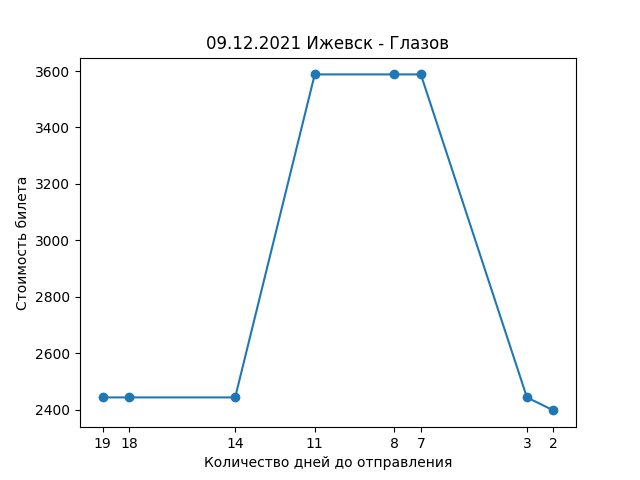
\includegraphics[scale=0.5]{09122021}
	\caption{Поезд с наибольшей динамикой ценообразования 9 декабря 2021 года}
\end{figure}

\begin{figure}
	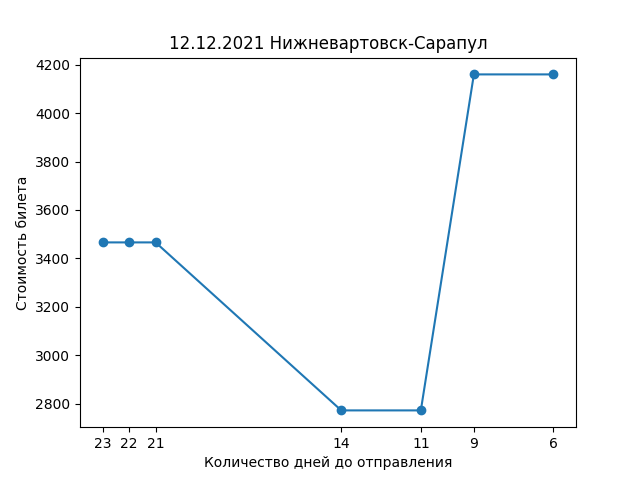
\includegraphics[scale=0.5]{12122021}
	\caption{Поезд с наибольшей динамикой ценообразования 12 декабря 2021 года}
\end{figure}

\begin{figure}
	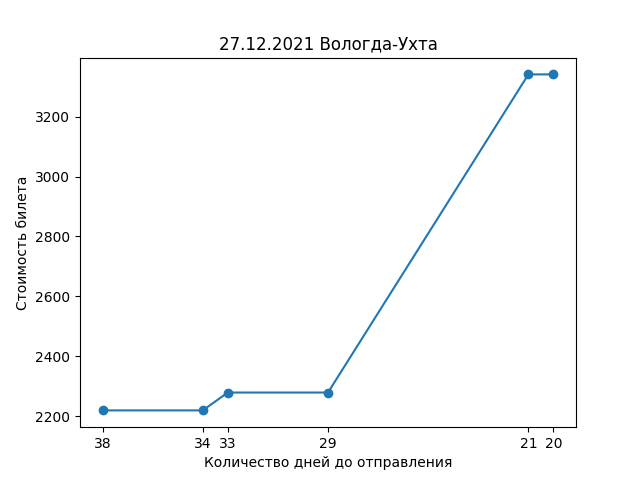
\includegraphics[scale=0.5]{27122021}
	\caption{Поезд с наибольшей динамикой ценообразования 27 декабря 2021 года}
\end{figure}

\begin{figure}
	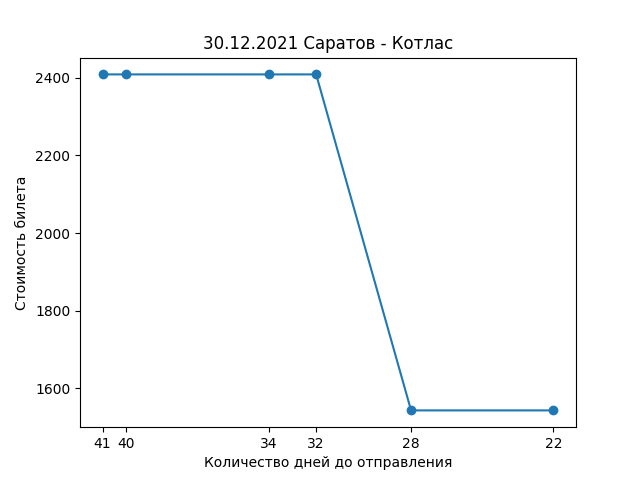
\includegraphics[scale=0.5]{30122021}
	\caption{Поезд с наибольшей динамикой ценообразования 30 декабря 2021 года}
\end{figure}

\begin{figure}
	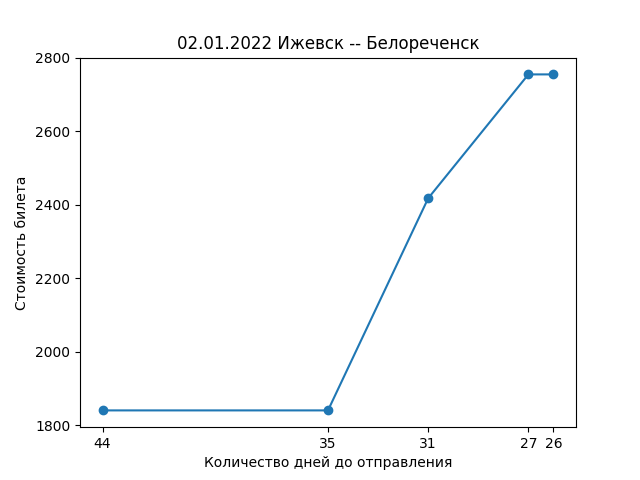
\includegraphics[scale=0.5]{02012022}
	\caption{Поезд с наибольшей динамикой ценообразования 30 декабря 2021 года}
\end{figure}

Проанализировав данные графики, можно заметить следующее:

\begin{itemize}
	\item В даты сильно повышенного спроса цены повышаются значительно раньше и сильнее, чем в даты с небольшим спросом
	
	\item Стоимость билета на поезд не обязана повышаться даже задолго до даты отправления. Можно заметить, что билеты на поезд, отправившийся 9 декабря, дорожали за 2 недели до отправления, а вот на поезд, отправившийся 12 декабря, наоборот подешевели
	
	\item За несколько дней до отправления (обычно за три дня), когда спрос спадает практически до нуля, а люди начинают сдавать билеты, эти самые билеты дешевеют. Данную особенность можно заметить, сопоставив приведённые выше графики с графиками зависимости количества свободных мест от числа дней до отправления.
\end{itemize}

Рассмотрим теперь графики зависимости числа свободных мест от количества дней до отправления.

\begin{figure}
	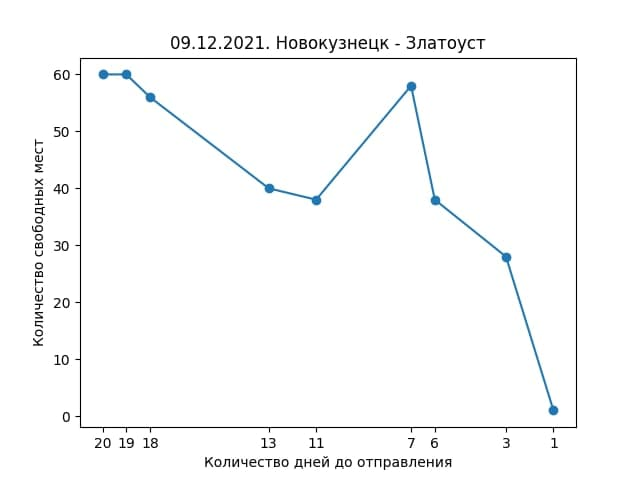
\includegraphics[scale=0.7]{09122021_seats}
	\caption{Поезд с наибольшей динамикой раскупаемости 9 декабря 2021 года}
\end{figure}

\begin{figure}
	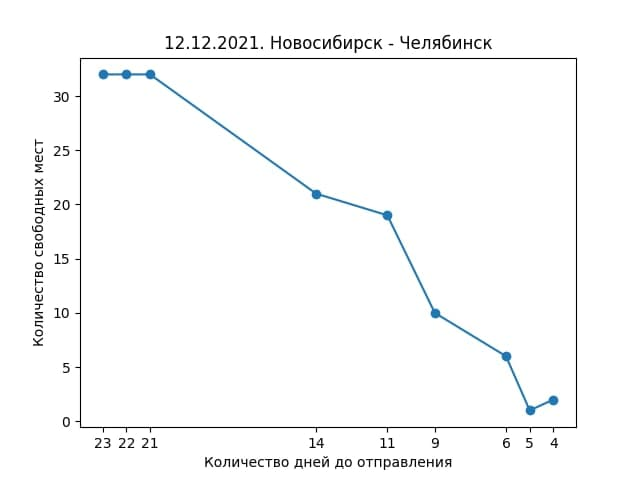
\includegraphics[scale=0.7]{12122021_seats}
	\caption{Поезд с наибольшей динамикой раскупаемости 12 декабря 2021 года}
\end{figure}

\begin{figure}
	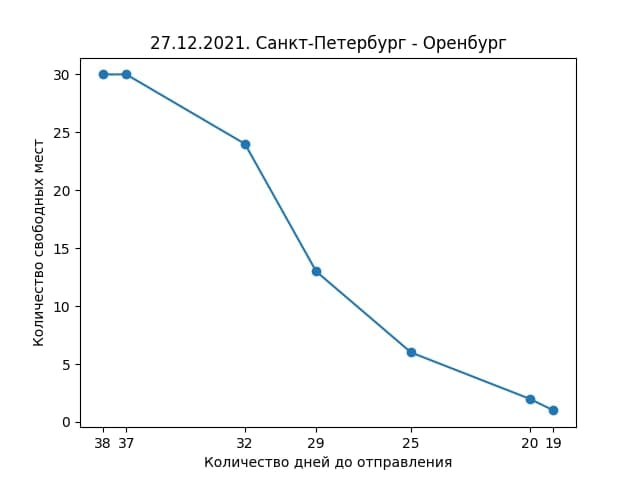
\includegraphics[scale=0.7]{27122021_seats}
	\caption{Поезд с наибольшей динамикой раскупаемости 27 декабря 2021 года}
\end{figure}

\begin{figure}
	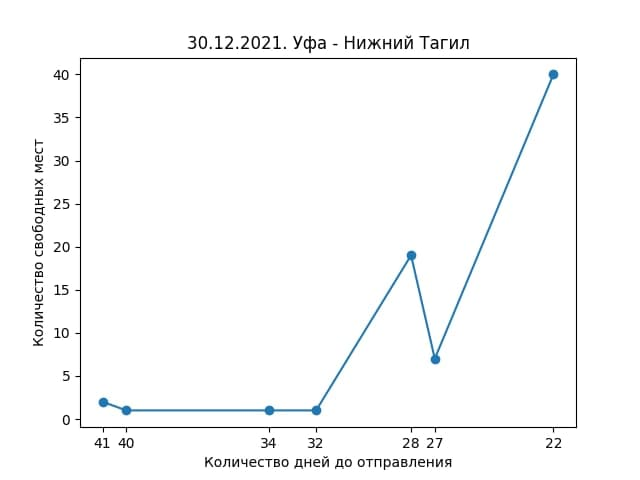
\includegraphics[scale=0.7]{30122021_seats}
	\caption{Поезд с наибольшей динамикой раскупаемости 30 декабря 2021 года}
\end{figure}

\begin{figure}
	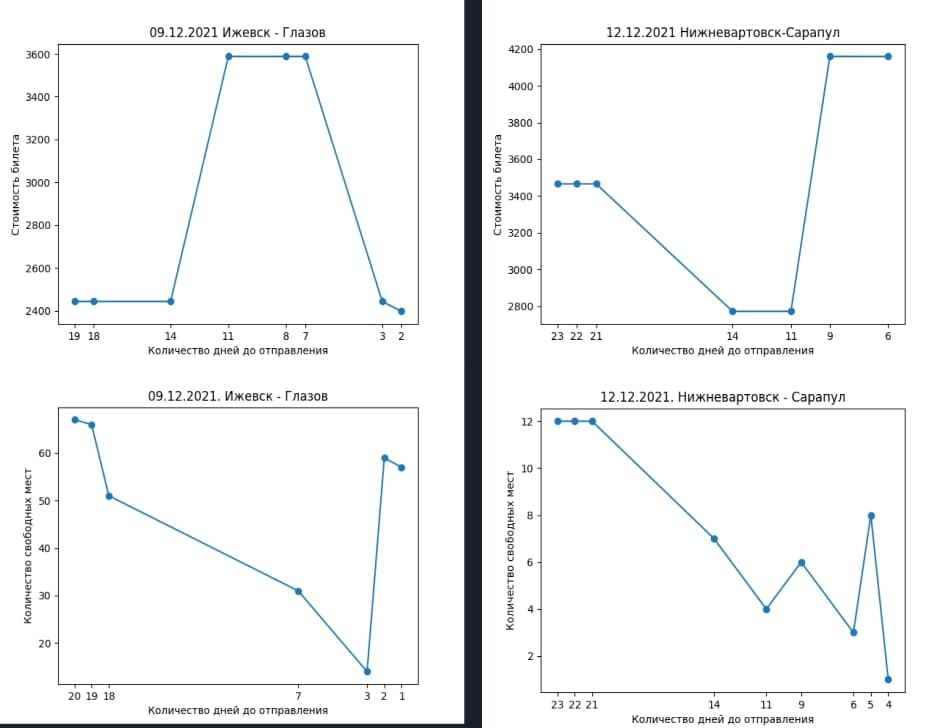
\includegraphics[scale=0.4]{4pict}
	\caption{Прямой связи между количеством свободных мест и стоимости билетов не наблюдается: в одном случае при высвобождении мест билеты подешевели, в другой ситуации при изменении спроса цена не менялась}
\end{figure}

\begin{itemize}
	\item В целом спрос на билеты либо линеен, то есть не заметны периоды наибольшей и наименьшей раскупаемости, либо же спрос лавинообразный, то есть билеты раскупают сразу же, как только появляются места. Такая динамика наиболее характерна для дат ажиотажного спроса, как в период праздников
	
	\item Зачастую за несколько дней до конца продаж билетов люди начинают сдавать билеты, что даёт некоторый шанс на покупку билета на дефицитный поезд перед отправлением
	
	\item При высоком спросе в ажиотажные даты РЖД добавляет дополнительные вагоны к поездам, причём иногда даже в несколько этапов. Это означает, что если в какой-то момент билетов на более дешёвый поезд или класс вагона нет, то не стоит сразу же покупать более дорогие билеты, а есть смысл подождать, пока РЖД добавит дополнительные вагоны
\end{itemize}
\section*{References}

Please number citations consecutively within brackets \cite{b1}. The 
sentence punctuation follows the bracket \cite{b2}. Refer simply to the reference 
number, as in \cite{b3}---do not use ``Ref. \cite{b3}'' or ``reference \cite{b3}'' except at 
the beginning of a sentence: ``Reference \cite{b3} was the first $\ldots$''

Number footnotes separately in superscripts. Place the actual footnote at 
the bottom of the column in which it was cited. Do not put footnotes in the 
abstract or reference list. Use letters for table footnotes.

Unless there are six authors or more give all authors' names; do not use 
``et al.''. Papers that have not been published, even if they have been 
submitted for publication, should be cited as ``unpublished'' \cite{b4}. Papers 
that have been accepted for publication should be cited as ``in press'' \cite{b5}. 
Capitalize only the first word in a paper title, except for proper nouns and 
element symbols.

For papers published in translation journals, please give the English 
citation first, followed by the original foreign-language citation \cite{b6}.

\begin{thebibliography}{00}
\bibitem{b1} G. Eason, B. Noble, and I. N. Sneddon, ``On certain integrals of Lipschitz-Hankel type involving products of Bessel functions,'' Phil. Trans. Roy. Soc. London, vol. A247, pp. 529--551, April 1955.
\bibitem{b2} J. Clerk Maxwell, A Treatise on Electricity and Magnetism, 3rd ed., vol. 2. Oxford: Clarendon, 1892, pp.68--73.
\bibitem{b3} I. S. Jacobs and C. P. Bean, ``Fine particles, thin films and exchange anisotropy,'' in Magnetism, vol. III, G. T. Rado and H. Suhl, Eds. New York: Academic, 1963, pp. 271--350.
\bibitem{b4} K. Elissa, ``Title of paper if known,'' unpublished.
\bibitem{b5} R. Nicole, ``Title of paper with only first word capitalized,'' J. Name Stand. Abbrev., in press.
\bibitem{b6} Y. Yorozu, M. Hirano, K. Oka, and Y. Tagawa, ``Electron spectroscopy studies on magneto-optical media and plastic substrate interface,'' IEEE Transl. J. Magn. Japan, vol. 2, pp. 740--741, August 1987 [Digests 9th Annual Conf. Magnetics Japan, p. 301, 1982].
\bibitem{b7} M. Young, The Technical Writer's Handbook. Mill Valley, CA: University Science, 1989.
\end{thebibliography}
\vspace{12pt}
\color{red}
IEEE conference templates contain guidance text for composing and formatting conference papers. Please ensure that all template text is removed from your conference paper prior to submission to the conference. Failure to remove the template text from your paper may result in your paper not being published.

\end{document}
